%%%
%
% $Autor: Wings $
% $Date: 2024-10-31 11:15:45Z $
% $File: file.tex $
% $Version: 1 $
%
% Project: 
%
%%%


\chapter{Supraplate}

\section{Verwendung der NFC-Schnittstelle}
Der SupraNano ist ein passiver Hochfrequenz transponder (HF), der auf der Near Field Communication (NFC) Technologie gemäß ISO/IEC 14443 basiert. Ein kritisches Merkmal ist die Integration einer elektromagnetischen Schirmung oder spezieller Ferrit Inlays, die den Betrieb auf metallischen Oberflächen (On Metal Funktionalität) ermöglicht.

In konventionellen NFC-Anwendungen führen metallische Untergründe durch Wirbelstrominduktion zur Auslöschung des magnetischen Haufelders.
Das System fungiert als physischer Ankerpunkt für dezentrale Datenbanksysteme. Die Datenübertragung erfolgt via NDEF (NFC Data Exchange Format), wodurch eine plattformunabhängige Kommunikation realisiert wird. \cite{yoke:2025}
%\cite{}Datenblatt Schraube
\begin{itemize}{
 \item Schnittstellen-Offenheit: Der Transponder ist nicht an ein proprietäres Ökosystem gebunden. Er unterstützt die herstellerübergreifende Kommunikation mit mobilen Endgeräten (Android iOS) sowie industriellen Handlesegeräten.

\item Software Integration: Die Konnektivität ist sowohl für die RiConnect Infrastruktur als auch für beliebige ERP- oder Instandhaltungs-Systeme von Drittanbietern via API Schnittstellen oder direkter URL Umleitung optimiert. \cite{yoke:2025}
} \end{itemize}


\section{Supraplate}

\subsection{Beschreibung Supraplate}

	Digitale Typenschilder stellen eine bahnbrechende Lösung dar, die sowohl in den Vereinigten Staaten als auch in der Europäischen Union die Einhaltung gesetzlicher Vorschriften gewährleistet und die Verwaltung durch IoT-Technologie verbessert.
	In der EU schreiben Richtlinien wie die Maschinenrichtlinie und die Arbeitsmittelrichtlinie eine eindeutige Kennzeichnung von Geräten und Sicherheitsbeschilderung vor. Digitale Typenschilder vereinfachen die Einhaltung der Vorschriften, indem sie wichtige Informationen wie Herstellerangaben, Modellnummern und CE-Kennzeichnungen digital anzeigen und so für eine Sichtbarkeit und Klarheit sorgen, die den EU-Standards entsprechen.
	In ähnlicher Weise verlangen die OSHA-Vorschriften in den USA eine wirksame Sicherheitskennzeichnung und Gefahrenkommunikation. 
	Digitale Typenschilder erfüllen nicht nur diese Anforderungen, sondern ermöglichen auch Echtzeit-Aktualisierungen und Fernüberwachung über IoT-Konnektivität. Dies stellt sicher, dass Sicherheitsinformationen aktuell und zugänglich bleiben, was die Sicherheit am Arbeitsplatz und die Einhaltung von Vorschriften verbessert.

	Durch den Einsatz von IoT-Technologie bieten digitale Typenschilder Vorteile, die über herkömmliche statische Etiketten hinausgehen. Sie bieten dynamische Verwaltungsfunktionen und ermöglichen proaktive Wartungswarnungen, Ferndiagnosen sowie die Überwachung der Einhaltung von Vorschriften. Dieser digitale Ansatz vereinfacht nicht nur die Einhaltung gesetzlicher Vorschriften, sondern verbessert auch die betriebliche Effizienz und Sicherheit sowohl in den USA als auch in der EU.
	Zusammenfassend stellen digitale Typenschilder einen entscheidenden Fortschritt bei der Einhaltung gesetzlicher Vorschriften und im Management dar, da sie sich nahtlos an US-amerikanische und EU-Standards anpassen und gleichzeitig die Möglichkeiten des IoT. \cite{yoke:2025}

\subsection{Merkmale}
\begin{itemize}{
\item NFC fähiges Mobilgerät oder Smartphone
	(iOS 14 oder höher erforderlich bzw. Android 12 oder höher erforderlich) kann als Lesegerät verwendet werden.
\item Korrosionsbeständiger Aluminium. 
\item Erfüllt die Anforderungen des US-Militärstandards MIL-STD-810H.\ref{MIL}
\item Erfüllt die Stoßfestigkeitsklasse IK10.\ref{IK}
\item Erfüllt die höchste Schutzklasse IP68 für Staub- und Wasserdichtigkeit. \ref{IP}
\item Einzigartiges Design der proprietären Wafer-Antennen-Chip-Konstruktion.
\item Patente in mehreren Ländern.
\item Durch die Verwendung der Supra Digital Chips in Verbindung mit einer Asset-Management-Anwendung eines Drittanbieters lassen sich Produktrückverfolgbarkeit, Herstellerauthentifizierung und digitalisierte Produktinformationen realisieren.
\item Patent in mehreren Ländern.\ref{Patent}

} \end{itemize}

\begin{center}
	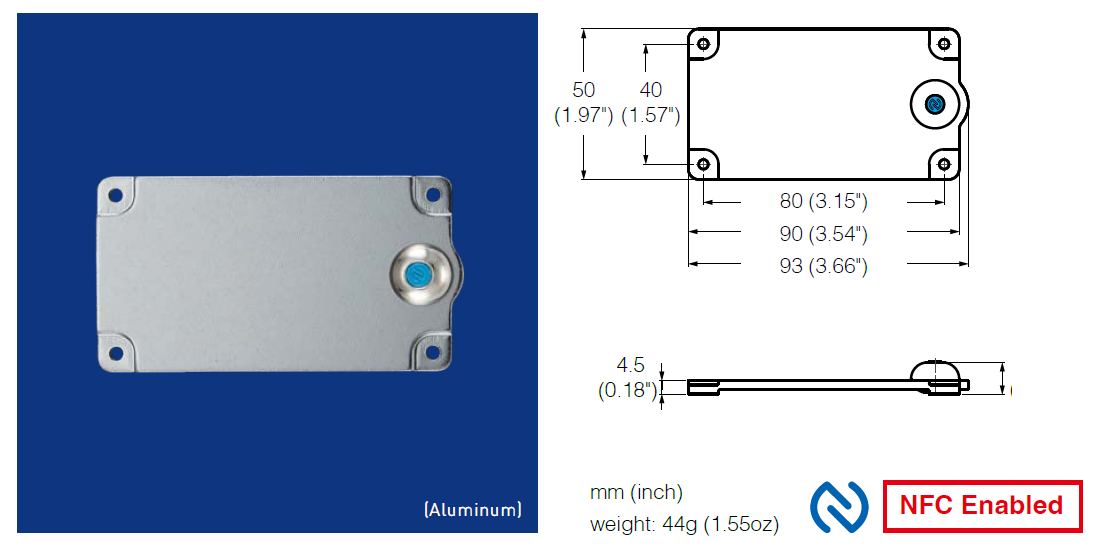
\includegraphics[width=\textwidth]{../../Images/Supra/SupraPlate.png}
	\captionof{figure}{Maße der Supra Plate}
	\label{pic:SupraPlate}
\end{center}

	In Abbildung \ref{pic:SupraPlate} ist die technische Zeichnung sowie eine perspektivische Ansicht des Bauteils dargestellt. Das Bild zeigt einen Sechskantschraubbolzen mit den Abmessungen 25mm (0,98") in der Gesamtlänge und einer Schaftlänge von 19,05mm (0,75").Dieses Bild verdeutlicht zudem die Kopfgeometrie, welche einen Durchmesser von 12,7mm (0,5") aufweist. Aus der Darstellung geht hervor, dass das Bauteil mit einem 5/16 - 18UNC Gewinde versehen ist. Hinsichtlich der Massenbilanz ist in der Abbildung ein Gesamtgewicht von 10,4 g (0,36oz) spezifiziert.
%https://www.google.com/url?sa=t&source=web&rct=j&opi=89978449&url=https://cms.yoke-europe.eu/uploads/Supra_Digital_Chip_Katalog_6ce294b388.pdf&ved=2ahUKEwijioqOs7GUAxVn_7sIHS0LByIQFnoECBoQAQ&usg=AOvVaw3nNXsRp-Gn6jiGbBH2EhU1

\begin{table}[h!]
	\caption{Nachfolgende Tabelle (\ref{SupraPlate}) zeigt die im Datenblatt \cite{yoke:2025} entnommen technischen Eigenschaften der Supra Plate.}
	\begin{center}
		\begin{tabular}{|l|l|}
			\hline
			\textbf{Parameter} &\textbf{Detail} \\
			\hline
			Funktionalität &  	\\
			\hline
			RF Protokoll & ISO 15693 	\\
			\hline
			Betriebsfrequenz & 13,56MHz 	\\	
			\hline
			Speicherkonfiguration  & UID 16 Bit, Benutzerdaten 2 KB 	\\	
			\hline
			Lese-/Schreibfähigkeit & Lesen / Schreiben  	\\	
			\hline
			Leistung &   	\\	
			\hline
			Lesereichweite & max. 5mm 	\\	
			\hline
			Ausrichtung  & Lesung von der Vorderseite \\	
			\hline
			IP-Schutzklasse & IP68 \\	
			\hline
			Physikalische Eigenschaften &   \\	
			\hline
			Werkstoffe & PA 6 + 30 GF, Aluminium \\	
			\hline
			Befestigungssystem & Universell einsetzbar \\
			\hline
			Farbe Tag & Türkisblau 	\\	
			\hline
			Farbe Gehäuse & Aluminium (eloxiert) 	\\	
			\hline
			Betrieb &  	\\	
			\hline
			Maximale Umgebungstemperatur & 125 °C / 257 °F 	\\	
			\hline
			Minimale Betriebstemperatur & -30 °C / -22 °F	\\	
			\hline
			Maximale Dauerbetriebstemperatur  & 125 °C / 257 °F 	\\	
			\hline
			Minimale Dauerbetriebstemperatur & -30 °C / -22 °F	\\	
			\hline
			Wasser- und eisbeständig & Ja \\	
			\hline
			\end{tabular}
		\label{SupraPlate}
	\end{center}
\end{table} 
%https://www.google.com/url?sa=t&source=web&rct=j&opi=89978449&url=https://cms.yoke-europe.eu/uploads/Supra_Digital_Chip_Katalog_6ce294b388.pdf&ved=2ahUKEwijioqOs7GUAxVn_7sIHS0LByIQFnoECBoQAQ&usg=AOvVaw3nNXsRp-Gn6jiGbBH2EhU1

\subsection{MIL STD 810}

\label{MIL}
Der MIL STD 810 ist ein Standard aus dem US-Militär. Die Norm spezifiziert die Umwelt-Testbedingungen, welche militärische Geräte unbeschädigt aushalten müssen, wie z.B. Regenwasser, Luftfeuchtigkeit, Schock, Vibration, Staub und Schimmelbefall. Hersteller von militärischer Ausrüstung führen diese Tests durch, um die Einhaltung des Standards zu demonstrieren.\cite{Heinen:2026} %\cite{}https://heinen-elektronik.de/glossar/mil-std-810/#was-ist-mil-std-810

\subsubsection{Welche Aussagekraft hat MIL STD 810?}

Die Bedeutung von MIL STD 810 liegt in seiner Rolle als Maßstab für die Haltbarkeit und Zuverlässigkeit von Ausrüstung unter extremen Bedingungen. Obwohl die Einhaltung des Standards nicht garantiert, dass ein Gerät allen aufgeführten Bedingungen getestet wurde, bietet sie eine wichtige Orientierungshilfe für Hersteller und Abnehmer. Für genauere Informationen über die Beständigkeit eines spezifischen Geräts wird auf die angegebene IP-Schutzart verwiesen.\cite{Heinen:2026}
%\cite{}https://heinen-elektronik.de/glossar/mil-std-810/#was-ist-mil-std-810

\subsection{IP 68 Standart}

\label{IP}
Die Prüfung der IP-Schutzart ist ein standardisiertes Verfahren, mit dem der Schutzgrad eines Gehäuses gegen das Eindringen von Fremdkörpern (z. B. Staub) und Feuchtigkeit bewertet wird. Der IP-Code (Ingress Protection Code) ist ein international anerkannter Standard (definiert durch die Normen IEC 60529 und ISO 20653), der den Schutzgrad von elektrischen Geräten und Gehäusen klassifiziert und bewertet.\cite{IB-Lenhardt:2026}

Der IP-Code besteht aus zwei Ziffern, von denen jede einen bestimmten Schutzgrad angibt:
\begin{itemize}{
	\item Die erste Ziffer steht für den Schutz gegen feste Gegenstände, wie Staub und Partikel, auf einer Skala von 0 bis 6.
	
	\item Die zweite Ziffer steht für den Schutz gegen Flüssigkeiten, wie z. B. Wasser, auf einer Skala von 0 bis 9.
}\end{itemize}


\begin{center}
	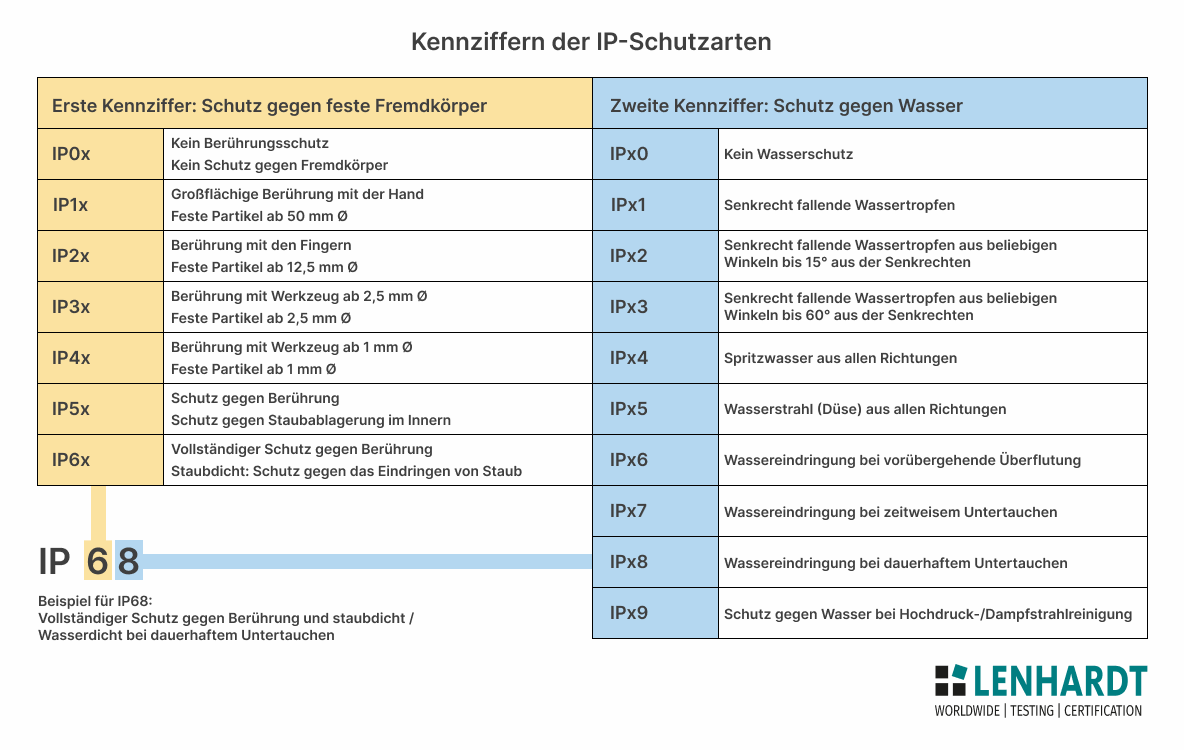
\includegraphics[width=\textwidth]{../../Images/Supra/IP.png}
	\captionof{figure}{Beispiel der IP Zertifizierung \cite{IB-Lenhardt:2026}}
	\label{pic:IP}
\end{center}

In der Abbildung \ref{pic:IP} wird die hierarchische Struktur der IP-Kennziffern tabellarisch gegenübergestellt. Die Grafik dient als Referenzmodell für die praktische Anwendung der Normen IEC 60529 und ISO 20653. Dieses Bild verdeutlicht die spezifischen Anforderungen der beiden Kennziffern: Linke Spalte (Erste Kennziffer): Hier wird die Skala für den Schutz gegen feste Fremdkörper visualisiert. Sie reicht von IP0x (kein Schutz) bis IP6x (vollständiger Berührungsschutz und staubdicht). Die Grafik zeigt auf, dass mit steigender Ziffer der Partikeldurchmesser abnimmt, gegen den das Gehäuse resistent ist (von $50\,\text{mm}$ bei IP1x bis hin zum Staubschutz bei IP6x).Rechte Spalte (Zweite Kennziffer): Diese Spalte klassifiziert den Schutzgrad gegen Wasser. Die Skala erstreckt sich von IPx0 bis hin zu IPx9, was den Schutz gegen Hochdruck- und Dampfstrahlreinigung definiert. Die Tabelle differenziert hierbei präzise zwischen verschiedenen Einwirkungsarten wie Tropfwasser (IPx1), Spritzwasser (IPx4), Strahlwasser (IPx5) und dem Untertauchen (IPx7/IPx8). Am Beispiel der Schutzart IP68 (unten links in der Abbildung markiert) wird die Kombination beider Werte anschaulich erklärt: Die Ziffer „6“ steht für ein staubdichtes Gehäuse, während die „8“ den Schutz gegen dauerhaftes Untertauchen zertifiziert. Diese visuelle Aufbereitung ermöglicht eine schnelle Identifikation des notwendigen Schutzgrades für spezifische Einsatzumgebungen elektrotechnischer Komponenten.\cite{IB-Lenhardt:2026}

%\cite{}https://ib-lenhardt.com/de/testen/ip-schutzart-pruefung?campaignid=21272639027&device=c&gad_source=1&gad_campaignid=21534526215

\subsection{IK 10 Standart}

\label{IK}
Die IK-Schutzklasse oder Stoßfestigkeit ist eine Klassifizierung, die den Schutzgrad eines elektrischen Geräts gegen äußere mechanische Einwirkungen, wie Stöße und Schläge bewertet. Die IK Schutzart wird durch eine Ziffer von IK00 bis IK11 angegeben, wobei IK11 den höchsten Schutzgrad darstellt. Je höher die Ziffer, desto widerstandsfähiger ist das Gerät gegen solche Einwirkungen.

Die bei den Produkten von Auer Signal gängigsten Schutzarten sind IK08 und IK09. Die Schutzart unserer Signalgeräte finden Sie auf unserer Website unter den technischen Daten des jeweiligen Produkts. Zusätzlich sind sie mit dem untenstehenden Zeichen und dem entsprechenden IK Code auf der Produktseite gekennzeichnet.\cite{Auer:2026} %\cite{}https://www.auersignal.com/de/technische-informationen/normen-kennzeichnungen/ik-schutzklasse/

\subsubsection{Unterschied IP gegen IK Zertifizierung}

Die IP-Schutzart (International Protection bzw. Ingress Protection) bezieht sich auf den Schutz gegen das Eindringen von Feststoffen und Flüssigkeiten in ein Gehäuse. Sie besteht aus einer Kombination von Buchstaben und Zahlen, die den Schutzgrad gegenüber Fremdkörpern und Wasser angeben. Die IK-Schutzklasse hingegen bewertet die Stoßfestigkeit gegen mechanische Einwirkungen. Diese beiden Schutzarten sind unabhängig voneinander und decken unterschiedliche Aspekte der Gerätesicherheit ab.

Die IK-Schutzart ist eine entscheidende Kennzeichnung, um sicherzustellen, dass elektrische Geräte und Gehäuse den erforderlichen Schutz gegen äußere mechanische Einwirkungen bieten. Dies trägt dazu bei, die Sicherheit von Personen und die Lebensdauer der Geräte zu gewährleisten, insbesondere in Umgebungen, in denen mechanische Belastungen auftreten können. Die Auswahl der richtigen IK-Klassifizierung hängt von der vorgesehenen Anwendung und Umgebung ab. \cite{Auer:2026}

\section{Further Readings}

\subsection{Patent}
\label{Patent}
\begin{itemize}{
		\item Deutsches Patent:		602018032891.2
		\item Taiwan Patent: 		M573545
		\item Taiwan-Patent:		I638765
		\item China-Patent:			ZL 201821589819.6
		\item China-Patent:			ZL 2017 1 0821524.0
		\item Japan-Patent:			3219858
		\item Japan-Patent:			3220091
		\item US-Patent:			10607128
		\item US-Patent:			10235617
		\item US-Patent:			11305844
		\item Italienisches Patent:	3627396
		\item Britisches Patent:	3627396
		
}\end{itemize}
\cite{yoke:2025}
